
\chapter{基于MPI的形态学图像处理}
\section{实验目的与要求}
\begin{enumerate}
    \item 掌握使用MPI进行并行编程设计和性能优化的基本原理和方法
    \item 使用MPI实现形态图像处理操作的并行算法
    \item 对程序执行结果进行简单的分析和总结
    \item 将其与Lab2和Lab3的结果进行比较
\end{enumerate}

\section{算法描述}
\par 对于MPI而言,由于其编程框架与OpenMP是不同的,因此需要使用不同的方法。由于在计算蚀刻以及膨胀时要使用一个像素周围的所有像素,如图\ref{fig:overlap}所示,因此如果使用\lstinline{MPI_Scatter}进行数据的分散则需要考虑分块边缘重叠的部分,实际上加大了程序编写的复杂度,而OpenMP和pthread程序由于是基于内存共享模型的因此不存在这一问题。而且由于需要对于重叠的部分进行额外的复制,若使用Scatter进行分散因此实际上降低了程序的性能。出于以上的考虑,直接使用Bcast将整张图片进行广播。

\begin{figure}[htpb]
    \centering
    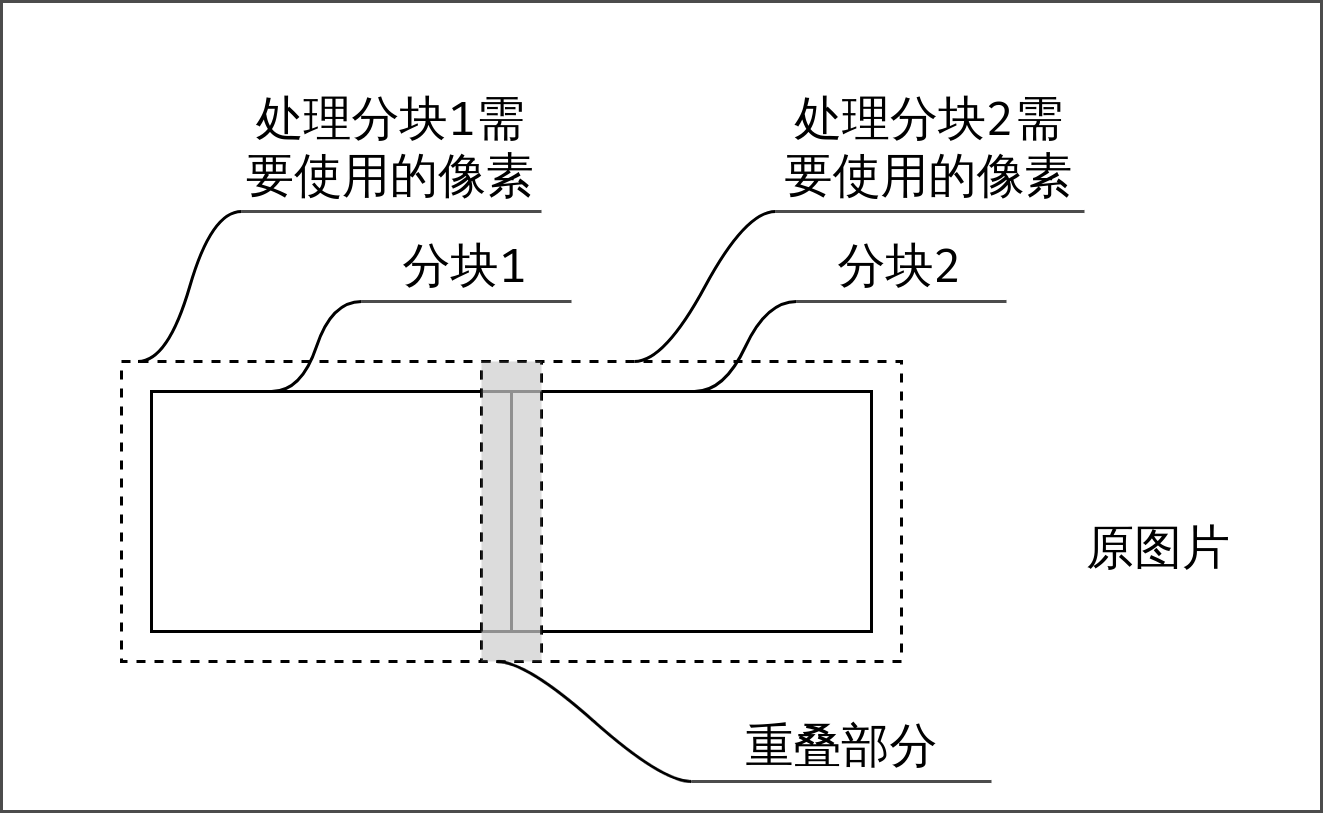
\includegraphics[width=0.6\linewidth]{overlap.png}
    \caption{两个分块的重叠部分}
    \label{fig:overlap}
\end{figure}

\par 将整张图片进行广播后,每个进程根据总的进程数量处理自己的分块,而新的分块方式如图\ref{fig:partition2}所示,在原图片的y方向上进行分块,除了主进程外每一个进程取与自己的编号相同的分块进行处理,最后使用\lstinline{MPI_Gather}对于处理的部分进行回收与拼接。由于在广播阶段广播整张图片,因此在处理时不需要考虑边缘重叠问题,此外,考虑到进程间数据传递的效率较线程间数据传递的效率低,因此不使用一个进程处理多个分块的方式,而是直接处理一个较大的分块直到处理完成。由于各个进程处理的数据量几乎一致,且处理逻辑是同质的,因此预计各个进程的处理时间不会相差太多。
\begin{figure}[htpb]
    \centering
    
\includegraphics[width=0.5\linewidth]{partition2.png}
    \caption{新的分块方式}
    \label{fig:partition2}
\end{figure}
\par 与pthread类似,在使用MPI进行并行处理时需要有一个主线程等待其他所有线程的完成,起到调度的作用。

\section{实验方案}
\par 依据实验思路进行代码的编写后编译进行测试。需要注意的是编译需要使用OpenMPI的包装编译器mpic++进行编译,在运行时也需要使用mpirun运行。多次改变进程数量后与前两次实验进行对比。

\section{实验结果与分析}
\par 使用4进程运行的结果如图\ref{fig:mpiOutput}所示,此输出在4个线程下运行得到。可以看到,程序运行时间为15.9s,相对于串行的加速比为\(44.2\div 15.9 = 2.77\),由于主线程不参与计算,因此这一结果与理想加速比3是比较接近的。
\par 对于其他进程数而言,由于有一个主进程,因此至少需要两个进程才能完整运行程序,而由于进程数不能超过物理内核数,因此实际测试的进程数只有2、3、4这3种情况,除掉主进程,有效进程数分别为1、2、3,与pthread和OpenMP进行对比的结果如图\ref{fig:mpiTrend}所示。可以看到其与pthread的性能相差无几。

\begin{figure}[htpb]
    \centering
    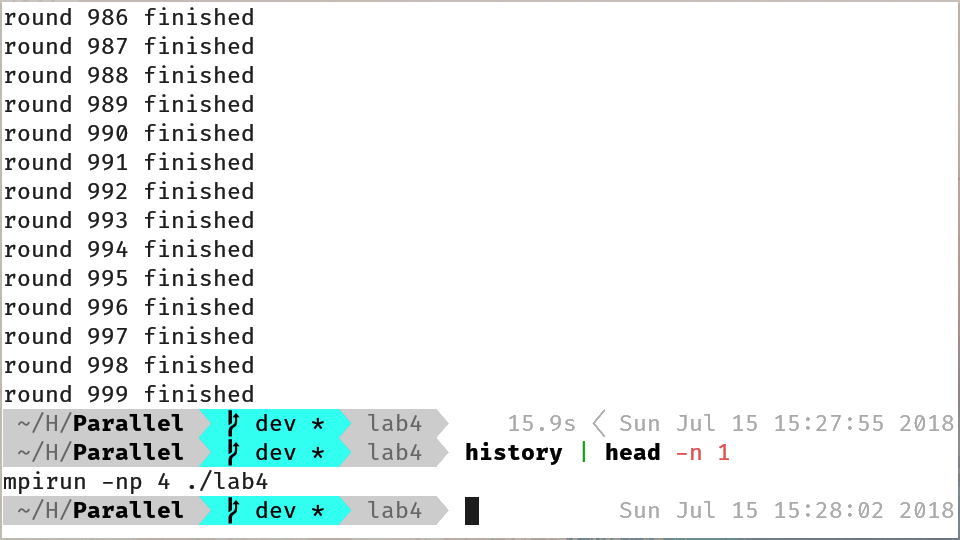
\includegraphics[width=0.8\linewidth]{mpiOutput.png}
    \caption{MPI程序输出}
    \label{fig:mpiOutput}
\end{figure}

\begin{figure}[htpb]
    \centering
    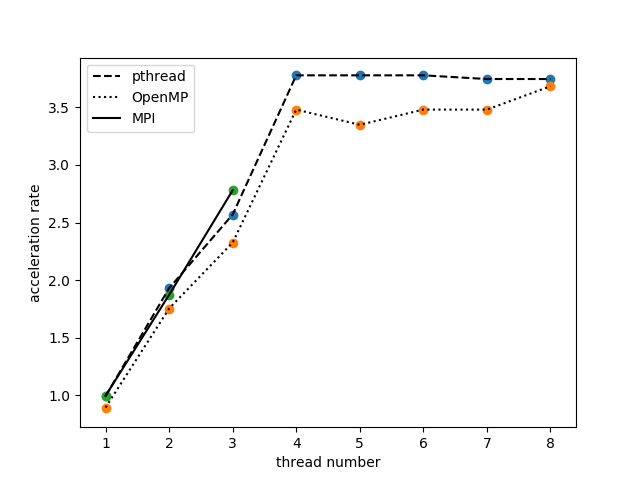
\includegraphics[width=0.8\linewidth]{mpiTrend}
    \caption{MPI程序与OpenMP、pthread程序的对比结果}
    \label{fig:mpiTrend}
\end{figure}


